\chapter{Languages for Graphics Programming}

A {\bf shader} is a program unit that runs on GPU; thus the GPU core is also
called as a shader. What a shader does is to determine how an object should
be drawn on the screen. Libraries like OpenGL or DirectX defines different
Shader APIs that can accept different inputs in the form of primitives
geometries and process them (e.g. real-time shadow, lighting, refraction, etc.)

The Shader APIs can be grouped into 2 classes: {\bf Pixel shaders} and {\bf
Vertex shaders}. This is better than fixed function pipeline, as it allows
developers to modify pixels and vertices dynamically.

The Shader APIs can be programmed using one of the 3 main shader languages: HLSL
(High-Level Shader Language, Sect.\ref{sec:HLSL}), C for Graphics (Cg) or GLSL
(OpenGL Shading Language). Depending on the hardware generation (graphics
cards), what the hardware can do are written in a particular version of the
specification (Sect.\ref{sec:shadermodel_specs}.
\begin{enumerate}
  \item Shader Model 1.1-1.4
  \item Shader Model 1.4
  \item Shader Model 2.0
  \item Shader Model 3.0
  \item Shader Model 4.0
  \item Shader Model 5.0
\end{enumerate}
Then, the shader APIs are developed based on these specifications. If you write
your games, for example, using APIs defined for the new specificaion; then the
game cannot run on older graphics cards.

First, you need to learn how a graphics image/video is processed
(Sect.\ref{sec:programming-with-gpu}).

\section{Graphical Programming with GPU (the road to unified architecture)}
\label{sec:programming-with-gpu}

GPU was first designed to handle rendering of images, which needs to go through a rendering pipeline -
Fig.\ref{fig:graph_pipeline}.

The images coming from different UI applications, and depending on their
z-depth, some may block the other partially or completely. This requires to GPU
to use different memory buffers - see video memory section
(Sect.\ref{sec:video-memory}).

By having a dedicated device for processing graphical output,  GPU free the CPU
from processing graphical data, the CPU can do other computational tasks more
efficiently.

\begin{mdframed}

The graphical data is a scene (e.g. image data) to be displayed on the screen.
There are multiple components (e.g. windows, objects) to be displayed on the
screen, one can hide the other (overlapping). Depending on how the user interact
with the objects, the new scene need to be generated and the final result is
sent to the 2D memory buffer for displaying it on the 2D screen fast enough.
Several algorithms have been developed to improve fast detection which region
is occluded. Also, in early times of
graphics, scence can only be in 2D, there is no depth effect (Z-depth). Thus the view in 2D can
be easily generated. To support Z-depth effect, 3D graphics cards have appeared,
and more sophisticated operations were required to map a 3D geometry into 2D
view on the screen, e.g. shading.


\end{mdframed}

The nature of image/video processing requires handling a large amount of data of
the same type (pixel, voxel). Also, as there is no accumulation of error like in
time-evolving simulator,  precision is not important for theses types of data
for displaying purpose.

At each stage of the rendering pipelines, early generations of GPU were limited
to running {\bf fixed-function pipeline} with 8-bit integer arithmetic
(Sect.\ref{sec:fixed-function-pipeline}). Later on, shaders are user-defined
functions that can be used at each stage of the rendering pipeline.



\subsection{Coordiante Systems}

To specify the relative spatial location between objects, we need to put them
into the same coordinate system. A person can observe the scene differently from
different standing position. Most 3D systems use {\bf Cartersian Coordinate
System}. There are other coordinate systems as well:
\begin{itemize}
  \item World Space (i.e. Model Space)
  \item Camera Space (i.e. Eye Space or View Space)
  \item Screen Space (i.e. Clip Space)
  \item Object Space
\end{itemize}

Object Space is the local coordinate  for a particular geometrical objects.

World Space is the coordinate where every objects are positioned, so that we can
tell the relative spatial positions between them.

In a real-world scene, depending where you stand, you may observe the scene at
different view. Similarly, in computer graphics, a particular view of the scene
is given based on the location of the ``eye'' or the virtual camera. To
understand how a scene is captured and being displayed on the screen, a virtual
camera concept is used. A virtual camera viewpoint is defined along with its
location from that a snapshot of the scene is capture. So, depending on the
orientation of the camera viewpoint, the angle of the light, different snapshots
of the scene is captured.


(1) A computer builds a complicated 3D object by breaking it down into a
set of simpler geometries that has a surface, and that surface is built from
vertices, edges, and triangles. \textcolor{red}{Why triangles?} they are really
quick and easy to compute.
The triangles are generated typically using Delaunay triangulation. 

(2) How can we process triangles? depending on the relative position and
orientation to the viewer, we take the transformed vertices and apply lighting
calculation for every light defined in the scene. As there are thousands of such
edges, vertices\ldots operations in a view, pipelining can be used to enhance
the performance. {\bf Pipelining} is also a common technique in CPU to enhance
the parallelizability of sequential applications by breaking the generic  task
into primitive tasks. 

(3) Rasterization: the geomtry is converted into pixels (to be displayed on
the screen). During rasterization, the triangles will be shaded and textured.

(4) Lightning? A big disadvantage at that time is that a GPU programmer had no
direct control over transformation, lightning and pixel rendering, because all
calculation models was fixed on the chip. These primitive functions are known as
{\bf fixed-function pipeline} (Sect.\ref{sec:fixed-function-pipeline}).

Modern GPU allows programmers to write code running on GPU. These binary
programs are called {\bf shader}, and the languages are called {\bf shader
programming languages} (Sect.\ref{sec:shader}). Regardless of which approach
being used (fixed-functin pipeline or shader programming languages), at lower
level, a number of intrinsic functions (APIs) need to be defined and supported
by the hardware. The specifications for these APIs are defined by two groups:
OpenGL and DirectX (Direct3D).

\subsection{How a ``view'' on the display is generated}
\label{sec:superf-viewp}

A snapshort of a (virtual) scene to be displayed is mathematically represented
by (1) vertices, (2) elementary geometries (e.g. triangles), (3) colors, (4)
lightning. Example: an image displayed on the screen is a snapshot of a virtual
scene which is defined by the geometry, orientation, material properties of
object surfaces and the position, characteristics of light sources,
Fig.\ref{fig:graphics_2D_3D}.


\begin{figure}[hbt]
 \centerline{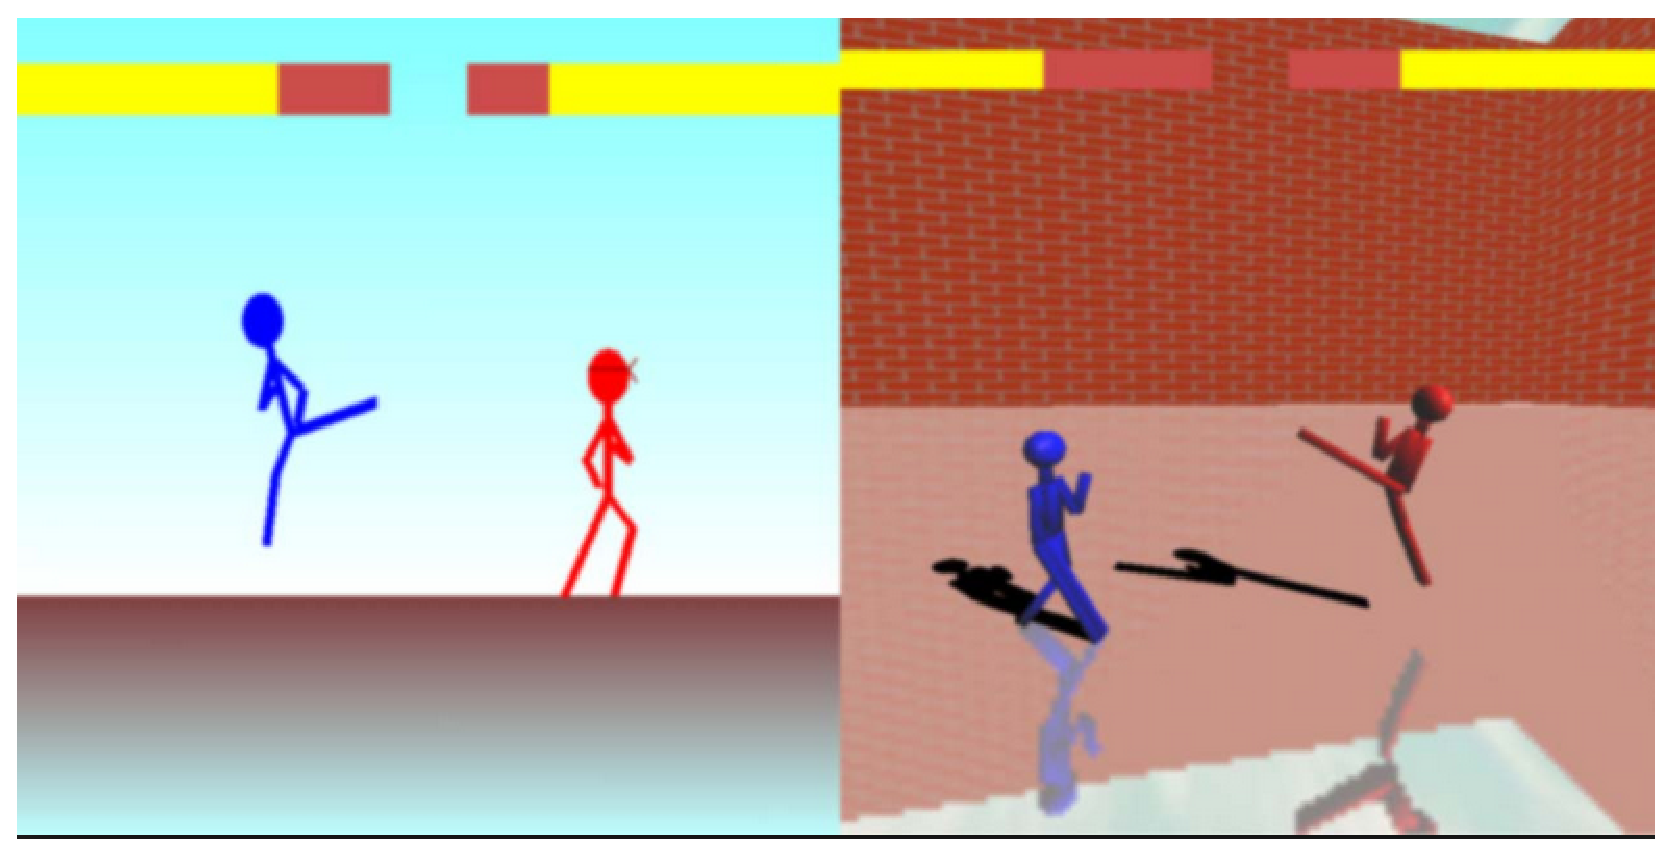
\includegraphics[height=5cm, angle=0]{./images/graphics_2D_3D.eps}}
 \caption{Graphics in 2D vs. 3D}
 \label{fig:graphics_2D_3D}
\end{figure}


To generate a graphic/picture/view, the objects (house, car, people,
animal\ldots) are put into a single ``world'', i.e. by scaling so that objects
have correct relatively aspect ratios and locations. In a physical world,
depending on the position of the ``viewer'', he/she can sense the objects
differently, e.g.  bigger or smaller, some parts are hidden or not.

\begin{framed}
  The ``viewer'' is modelled as a virtual camera, and a
  {\it scene view} is described by the location of a virtual camera, or
  ``camera'' angle, Fig.~\ref{fig:graph_virtual_camera}.
\end{framed}

\begin{figure}[hbt]
 \centerline{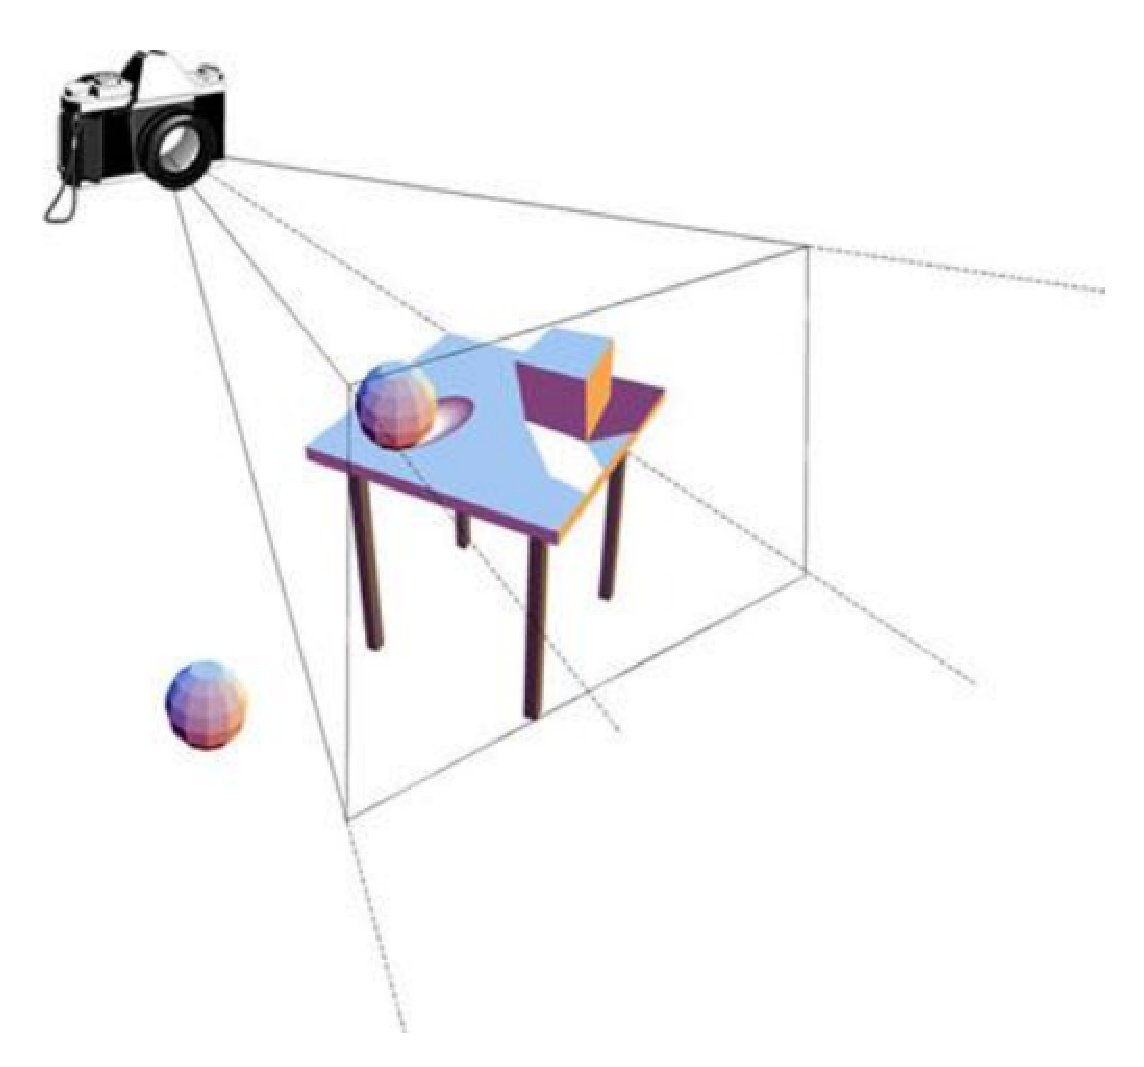
\includegraphics[height=5cm, angle=0]{./images/graphics_virtual_camera.eps}}
 \caption{Virtual camera}
 \label{fig:graph_virtual_camera}
\end{figure}

To facilitate the processing, a new coordinate system whose origin is
at the camera is
created\footnote{\url{http://alt.pluralsight.com/wiki/default.aspx/Craig.DirectX/CoordinateSystemsTutorial.html}}.
So, the GPU need to map objects from their own ``world'' coordinate to
``camera'' coordinates which goes through a number of steps.
\begin{itemize}
\item Depending on the location of the camera, several necessary
  transformations need to be done to move the objects from that world
  space to the view space, e.g.  rotated (spinning on an axis),
  translated (shifting along an axis), or scaled (made bigger,
  smaller, or even stretched/shrunk along a certain axis).

\item Depending on the view angle, some parts of the objects may be
  hidden (or occluded). Thus, the stage ``occlusion culling'' need to
  be performed to remove triangles that are hidden. During this stage,
  to create 3D effects, an important factor is the color and shadow
  effect, i.e. the system need to generate ``lighting'' or
  ``illumination'' effect to the scene, e.g. texturing, shadow mapping.
\end{itemize}

A 3D scene is often represented by triangular meshes filled with {\it color} or
{\it textures}. A texture is a 2D color image, stored in GPU memory. There are
two pipelines to improve graphical processing: {\bf task pipelines} and {\bf
data pipelines}. In data pipelines
\begin{enumerate}
  \item a stream of vertices (representing triangular meshes) is read from the
  CPU memory, and processed in parallel by the {\it vertex shaders} which do
  vertex processing tasks like projecting the geometry onto the image plane of
  the virtual camera, computing the surface normal vectors or generating 2D
  texture coordinates for each vertex.
  \item vertices are assembled into triangles to undergo {\it rasterization},
  i.e. the hardware unit that determines which pixels are covered by a triangle,
  and generate a {\it fragment} (a small data structure with information needed
  to update the pixel in the frame buffer)
  \item the streams of fragments is processed in parallel by the {\it fragment
  shaders} to compute the final colors and transparency fo the pixels. It may
  need to fetch textures, calculate lightning effects, determine occlusions,
  and define transparency.
\end{enumerate}

Other necessary operations involve:
\begin{itemize}
\item Rasterizing (by Raster Engine): converting geometry (an image
  described as a series of primitive shapes) into pixels (i.e. a
  raster image for output on a video display).
\item Pixel processing: depth tests, stencil tests, and other
  per-pixel operations.
\item Vertex processing:
\item Geometry processing: how to render a triangle
\end{itemize}

\subsection{APIs: OpenGL vs. DirectX (Direct3D)}

In the early days of GPU computing, the GPU could only be programmed using APIs
for graphics rendering, e.g. render complex 3D scene.

Both OpenGL and DirectX defines the APIs that can be used for graphical
processing. A GPU model is said to support (the graphics driver) one particular
version of OpenGL or DirectX if it has the dedicated hardware to run these APIs.
Typically, a GPU model support both standards for a given version
\begin{itemize}
  \item GPU during 2004: support DirectX 9 and OpenGL 2
  \item GPU during 2008: support DirectX 10 and OpenGL 3
  \item GPU during 2011: support DirectX 11 and OpenGL 4
\end{itemize}
The standards are designed with backward-compatibility in mind, so that an older
application can run on new GPU models.

The APIs are grouped in such a way that each can be run by a dedicated hardware
unit to do separated things (different type of shading tasks). As a result,
different names were given to the hardware units (Sect.\ref{sec:shader}). To
expose the APIs to user, Direct3D develop the so-called {\bf Shader Model}
(Sect.\ref{sec:shader_model}, Sect.\ref{sec:shadermodel_specs}). Each version
defines how advanced shading techniques are allowed to get on a graphics card.

With the evolution of GPU architecture, the discrimination between shaders are
removed. A single shader (or GPU hardware unit) can do any type of shading task.
This is called {\bf unified shader model} (in OpenGL) or {\bf Shader Model 4.0}
(in Direct3D 10). The unified shading architecture are used in Nvidia
CUDA-capable GPUs: Tesla, Fermi, Kepler, Maxwell. 


\subsection{Video memory}
\label{sec:video-memory}
\ref{sec:framebuffer}

The space complexity is two times the number of pixels because two arrays of
pixels are required, one for frame buffer and the other for the depth buffer.

Stencil and Z-buffers are part of the frame buffer, coupled to the color buffer. 
\url{https://unity3d.com/learn/tutorials/topics/best-practices/framebuffer}

\begin{enumerate}
  \item frame-buffer: Sect.\ref{sec:framebuffer}
  The framebuffer contains the depth, stencil, and color buffers.

In video animation, to switch from one frame to another smoothly,
double frame buffers is often used, i.e. the new frame is loaded into
the another frame buffer so that it doesn't affect the
currently-displayed frame. Then, the amount of memory for the buffer
is doubled, e.g. we need 15MB. Or even, triple buffering can be used.

So, why we need Graphics card with much more memory, like 128MB or
256MB... In deed, to generate better image, different techniques can
be used which may requires more memory. For example: FSAA (full-scene
anti-aliasing) render more pixels that a display use, and then average
them out to give a final smooth picture fitting to the display
device. And this memory increase when the Graphics process 3D image. 

In 3D data, there are additional special buffers: {\bf Z-buffer}, and
{\bf stencil buffer}. 
  
  \item Z-buffer (aka Depth-buffer method): \label{sec:z-buffer}

In a 3D scene, each pixel often associated with a given depth to represent a 3D scence on a 2D screen.


The z-buffer has the same internal data structure as an image, namely a
2d-array, with the only difference being that it stores a z-value for each
screen pixel instead of pixel data.
t has the same dimensions as the screen buffer, except when multiple z-buffers
are used, such as in split-screen rendering. It operates in screen-space and
takes as its input a projected image that originates from a projection of an
object to the screen. \url{https://en.wikipedia.org/wiki/Z-buffering}

When viewing a picture containing non transparent objects and surfaces, it is
not possible to see those objects from view which are behind from the objects
closer to eye. To get the realistic screen image, removal of these hidden
surfaces is must. The identification and removal of these surfaces is called as
the {\bf Hidden-surface problem}.


Z-buffer, which is also known as the Depth-buffer method is one of the commonly
used method for hidden surface detection. It is an Image space method.
Image space methods are based on the pixel to be drawn on 2D. For these methods,
the running time complexity is the number of pixels times number of objects.
 

  
In a 3d-rendering engine, when an object is projected on the screen, the depth
(z-value) of a generated pixel in the projected screen image is stored in a
buffer (the z-buffer or depth buffer). A z-value is the measure of the
perpendicular distance from a pixel on the projection plane to its corresponding
3d-coordinate on a polygon in world-space.

The Z-buffer is used to determine what's in front of what in the
rendered scene. 
\url{https://www.geeksforgeeks.org/z-buffer-depth-buffer-method/}
    
  \item stencil buffer: \label{sec:stencil-bufer} is used to mask out, i.e.
  determine what region to be rendered.
  For each pixel, there's a corresponding stencil value, and pixels can be
  conditionally modified/ignored depending on these values.
  So, stencil buffer is the buffer that controls which pixels can be modified
  when polygons are rendered.
  
  

In its original incarnation, a stencil buffer was a one-bit-per-pixel (i.e.
black or white, but no grays) framebuffer. You could render to it whatever you
wanted like any other framebuffer.
Then, later, you could use the contents of that buffer to "stencil" or mask out
when drawing to your regular buffer, i.e. a mask that allows some pixels
through, and stops other pixels being modified.


The stencil buffer is another piece of unnecessary-pixel-rendering-avoidance
technology.  Similar to z-buffer - like depth testing, stencil testing is a
true/false test (that's why single bit is needed for one pixel).
 

The depth buffer and stencil buffer often share the same area in the
RAM of the graphics hardware; with typically the ratio is 24 bits for Z-buffer +
8 bits for stencil buffer or, in the past, 15 bits for Z-buffer + 1 bit for
stencil buffer. Another variant is 4 + 24, where 28 of the 32 bits are used and 4 ignored.


In the simplest case, the stencil buffer is used to limit the area of rendering
(stenciling).
An example: Let's say you're making a driving game. You want to have a little
rear-view mirror onscreen that shows you what's behind the car. You'll need to
render a view pointing behind the car, but you only want to render that within
the little rounded rectangle of the rear-view mirror. The typical solution is:
\begin{verbatim}

Render the rounded rectangle shape to the stencil buffer.
Enable stencilling.
Render the backwards pointing view onto the regular buffer.
\end{verbatim}
The stencil will then mask it out so that you only draw into the shape of the mirror.

Now that render pipelines are much more flexible and programmable, stencil
buffers are used as just a generic 1-bit framebuffer that you can do whatever
you want with. Shadows are a common use case.

Due to the position of the stencil test in the graphics pipeline (which is
before pixel shading), stencil testing can be used to kill pixels that do heavy
shading work when they're not needed.
Often this can be done at a coarser granularity than just a single pixel eg. a
tile of pixels, so work can often be culled during the coarse rasterization
stages too.

More advanced usage of the stencil buffer makes use of the strong connection
between the depth buffer and the stencil buffer in the rendering pipeline.

\url{https://gamedev.stackexchange.com/questions/3770/what-is-the-purpose-of-the-stencil-buffer-more-precisely-what-is-a-stencil-in}
\end{enumerate}

The memory demand for GPU is more intensive when more tasks are shifted to
GPU. 


References:
\begin{enumerate}
\item \url{http://www.dansdata.com/gz014.htm}
\end{enumerate}


\subsection{framebuffer: how do pixels end up on the monitor?}
\label{sec:framebuffer}

For a 2D video display of size $X\times Y$ (in pixels), the amount of
memory required to store the whole-screen image is
\begin{lstlisting}
X * Y * number of bits per pixel
\end{lstlisting}
This block of memory is known as {\bf frame buffer}. The Graphics then
will feed the frame buffer to the digital-to-analog hardware to create
the image on the CRT monitor; or just simply send to the digital DVI
monitor. For example: 1600 by 1200 resolution, with 32 bit colour,
then that's a total of 61,440,000 bits for the whole display. Which is
7,680,000 bytes, which is 7,500 kilobytes, which is about 7.32
megabytes.


The image displayed on the monitor is stored in your computer’s video RAM on the
graphics card in a structure called a framebuffer.

A framebuffer is a portion of RAM containing a bitmap that drives a video
display.
The information in the buffer typically consists of color values for every pixel
to be shown on the display. The framebuffer (for GPU 0) is 
\begin{verbatim}
/dev/fb0
\end{verbatim}


The data in the video RAM can be generated by the GPU or by the CPU. 

\begin{verbatim}

RAM (framebuffer)     -------[read by DMA componnent]---->  Graphics card ---[VGA/HDMI/DVI cable]------> monitor
\end{verbatim}

The video RAM is continuously read out by a specialized DMA component on the
video card and sent to the monitor.
The signal output to the monitor is either an analog signal (VGA) where the
color components are sent through digital to analog converters before leaving
the card, or a digital signal in the case of HDMI or DVI.


\textcolor{red}{How large is framebuffer}: 1920x1080 display with 4 bytes per
pixel, you only need about 8 MB to store the image.


But the video RAM in your computer is probably many times that size. This is
because the video RAM is not only intended for storing the framebuffer. The
video RAM is directly connected to the GPU, a special purpose processor designed
for efficient 3D rendering and video decoding.

\textcolor{red}{HACK write to framebuffer yourself}:
/dev/fb0 acts like any other memory device in /dev and we can write to it like a file.

\begin{verbatim}
> cat /dev/urandom > /dev/fb0
-bash: /dev/fb0: Permission denied

> sudo cat /dev/urandom > /dev/fb0
-bash: /dev/fb0: Permission denied

> ls -al /dev/fb0
crw-rw---- 1 root video 29, 0 Apr  4 00:21 /dev/fb0

> sudo adduser seena video
> cat /dev/urandom > /dev/fb0
\end{verbatim}

\url{http://seenaburns.com/2018/04/04/writing-to-the-framebuffer/}

\subsection{Hardware Tessellation}
\label{sec:tessellation}

DirectX 11 support a new feature that requires a hardware unit for tessellation.
So any GPU that support DirectX 11 must have this programmable tessellation
unit. Simply, the job of tessellation is to add more detail to 3D objects, in
real-time.

\begin{framed}
  The process of rendering an object (of any complexity) from the
  geometric primitive is called {\bf tessellation}, as shown in
  Fig.~\ref{fig:graph_pipeline}. Traditionally, this operations is
  done by software.  DX11 standard has brought this task to the
  hardware (GF100 from Nvidia supports this new feature).
\end{framed}

Bassically, tessellation is the process of subdividing a surface into smaller
shapes, by recursively applying a subdivision rule to breaking down the surface
of an object into manageable polygons, e.g. increasing your polygon count to get
more detail, Fig.\ref{fig:Tessellation_example}. NOTE: To better display a
scene, we typically need much polygonal complexity closer to the viewer or
camera, and fewer polygons as distance from the camera increases.

Triangles or quadrilaterals are two commonly used polygons in drawing graphical
objects because computer hardware can easy manipulate and calculate these two
simple polygons. n object divided into quads and subdivided into triangles for
convenient calculation. Now, with the designated hardware unit, this process can
now be done 100\% at GPU level in hardware without a significant impact on
performance. The tessellation unit is programmable via two new shader
(introduced for tessellation in DirectX 11): {\bf Hull Shader} and the {\bf
Domain Shader}.

\begin{figure}[hbt]
  \centerline{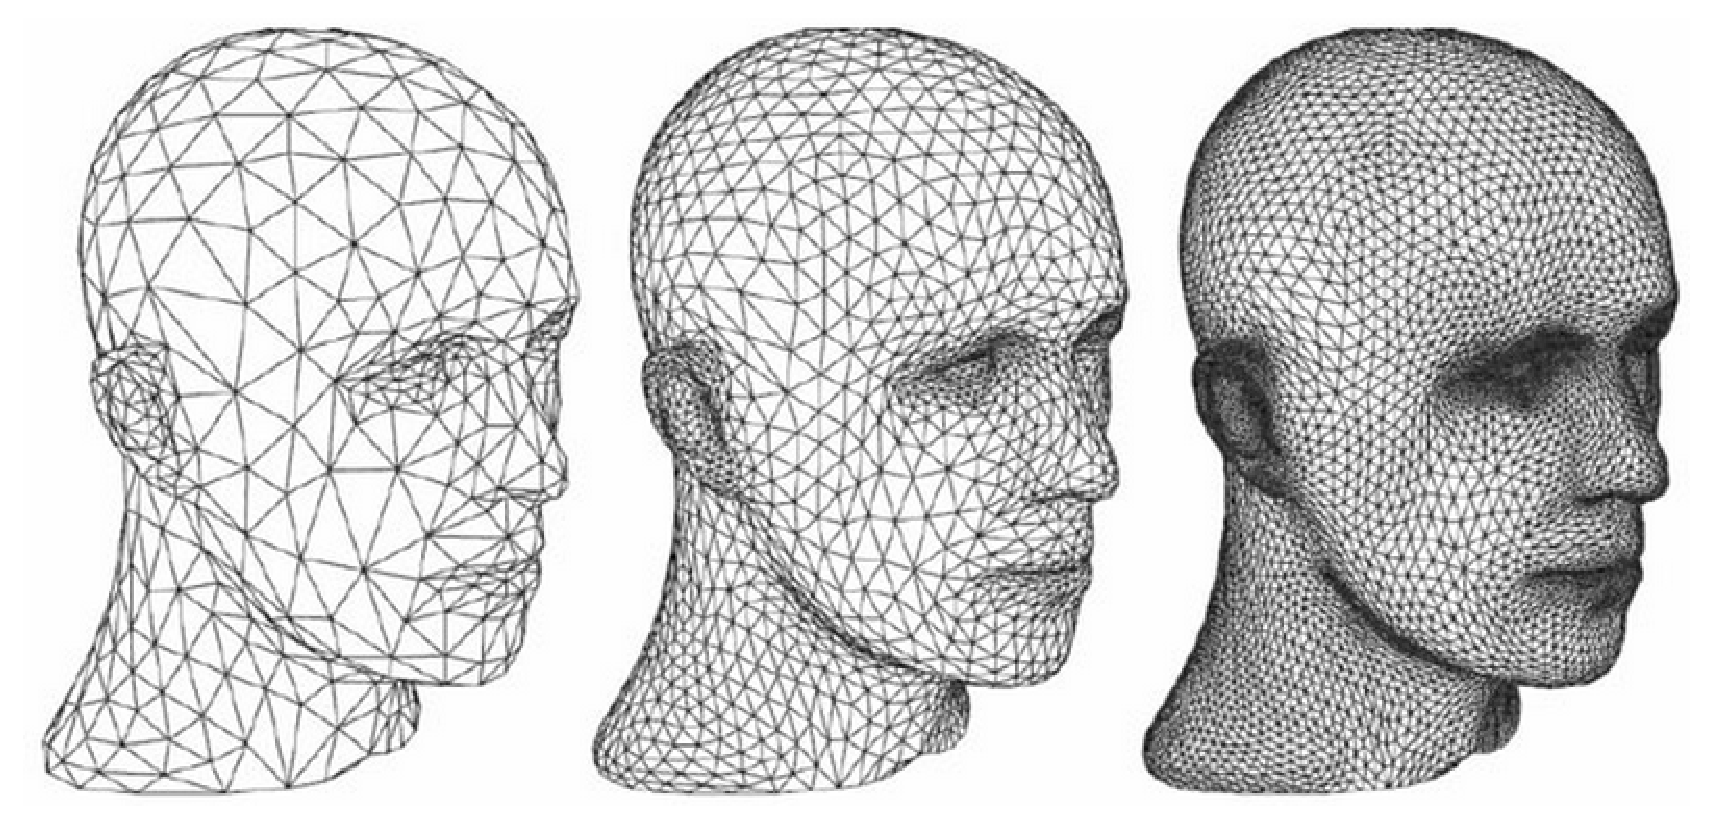
\includegraphics[height=5cm,
    angle=0]{./images/Tessellation_example.eps}}
\caption{An example of tessellation}
\label{fig:Tessellation_example}
\end{figure}


\subsection{Fixed-function pipelines: non-programmable GPU cores}
\label{sec:fixed-function-pipeline}

In early times, interacting with GPU can be done by calling some primitive
functions developed by hardware developers written in the drivers. Programmers
can call these APIs (these primitive functions) by passing data as the
parameters.
Date are different matrices or set certain parameters. This is the best that can
be done with the old chips design back in the day when the fixed pipeline was
the only option.


OpenGL expose features of the underlying graphics hardware to application
developers. These functions are part of OpenGL (in the early version) when
graphics hardware are NOT programmable.


With fixed-functions, what you can do is limited by the APIs, e.g. the
lightning is done by a call to a predefined function. Fixed-functions
works on 4 fundamental entities: vertices, primitives, fragments, and
pixels\footnote{\url{http://queue.acm.org/detail.cfm?id=1400197}}, the
green boxes in Fig.~\ref{fig:graph_pipeline2}. The process is described as
follows.

These primitive graphical functions operate on vertices, edges, and simple
geometry shapes to map them to a 2D framebuffer - Sect.\ref{sec:framebuffer} -
which is then flushed to the monitor screen (either analog or digital) for
display. 

\begin{framed}

  The term {\bf fixed-function} means the functions are hard-coded, the only
  ``customization'' is to pass different parameters.  They are characterized by
  functions calling between \verb!glBegin()! and \verb!glEnd()!. Its set is
  increasingly expanded from one generation to another. They become obsolete and
  was removed from OpenGL 3.1 which nows uses Shaders (Sect.\ref{sec:shader}).
  
  OpenGL 3.0 was the last revision of the specification which fully supported
  both fixed and programmable functionality. Even so, most hardware since the
  OpenGL 2.0 generation lacked the actual fixed-function hardware. Instead,
  fixed-function processes are emulated with shaders built by the system.
  
  \url{https://www.khronos.org/opengl/wiki/Fixed_Function_Pipeline}
\end{framed}


  \begin{enumerate}
  \item Objects are represented by {\bf geometric primitives}: points,
    lines, triangles, and polygons. Each one is defined by a set of
    vertices. So, in the very first step, the application need to
    provide a set of vertices descriptors. Based on this list, Vertex
    Generator (VG) prefetches vertex data from memory and construct a
    stream of vertex data record. Each record contain 3D (x,y,z)
    position of the vertex, as well as application-defined additional
    information like surface color, normal vector orientation

  \item Next step, Vertex Processing (VP) is application
    programmable. Each VB function take one vertex data record as input
    and produce one output vertex record. The ultimate purpose is to map
    3D scene to 2D image on the screen.

  \end{enumerate}

\begin{figure}

  \begin{minipage}[b]{0.5\linewidth} 

    \begin{enumerate}
      \setcounter{enumi}{2}
    \item Primitive Generation (PG) uses the vertex topology data provided
      by the application to group the vertices (output from VP) in an
      ordered stream of primitives. Each primitives is the concatenation
      from different output vertex records. This also define the order of
      primitives at output stream, i.e. which primitive is displayed first
      and next. However, this order can change. 

    \item Primitive Processing (PP) operates on the primitives to
      determine which primitives should be hidden. This may leads to
      generating more primitives. 

    \item Fragment Generation (FG) does the process {\bf rasterization},
      i.e. samples each primitive. Each sample is manifest as a {\bf
        fragment}. 
    \item Fragment Processing (FB) simulates the interaction of light with
      scene to determine the surface color and opacity at the fragment's
      sample point. This process makes heavy use of filtered lookups into
      large, parameterized arrays - known as 1D, 2D, 3D {\bf textures}. 

    \item Pixel Operations (PO) use each fragment's screen position to
      calculate and apply the fragment's contribution to output image's
      pixel values. It will examine the distance of fragments from the
      virtual camera and discards fragments that are blocked by closer
      ones. 

    \end{enumerate}
OpenGL/DirectX and
higher-level graphics libraries are those described in red boxes in
Fig.~\ref{fig:graph_pipeline2}. 

  \end{minipage}
%  \hspace{0.5cm}
  \begin{minipage}[b]{0.5\linewidth}
    \centerline{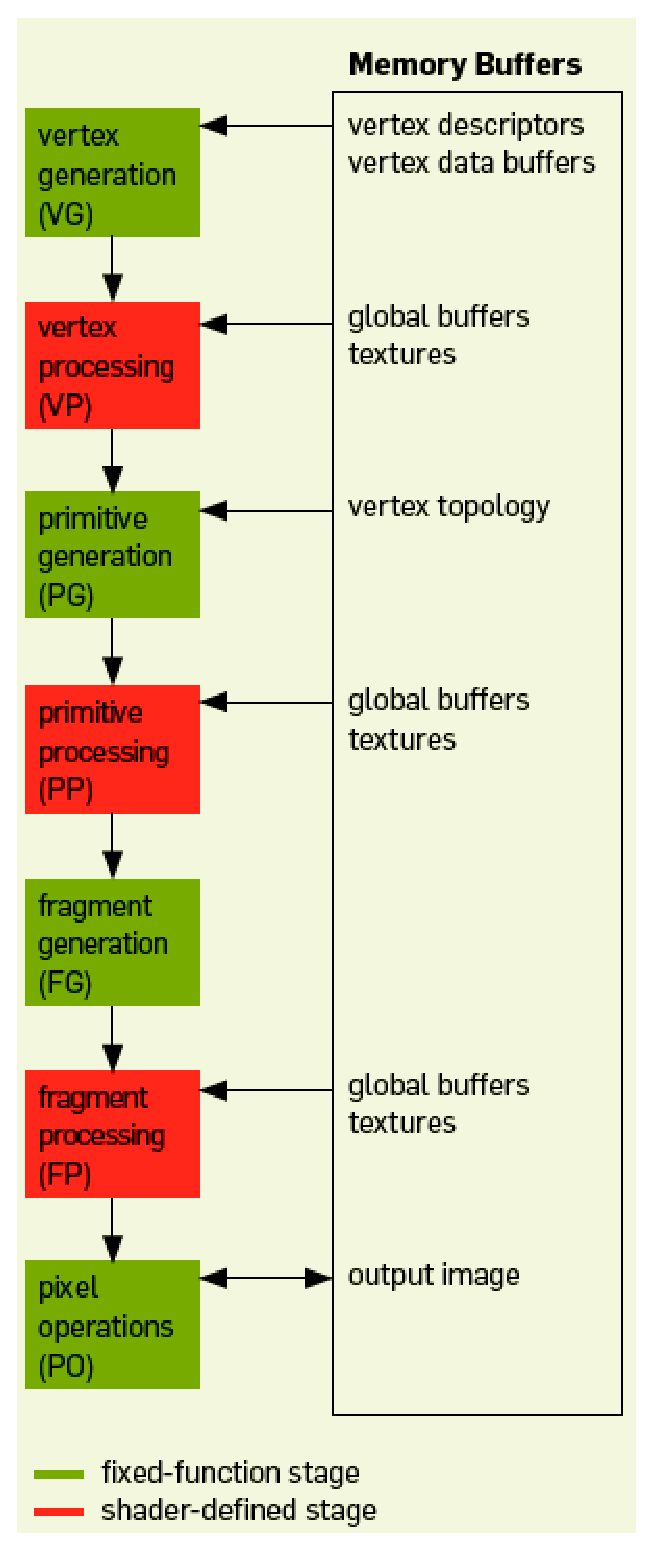
\includegraphics[height=15cm,
      angle=0]{./images/pipeline.eps}}
    \caption{A simplified graphics pipeline}
    \label{fig:graph_pipeline2}
  \end{minipage}
\end{figure}

% This will increase code usability as functions to process these
% primitives can be reused to manipulate objects of any complexity.


\begin{figure}[hbt]
  \centerline{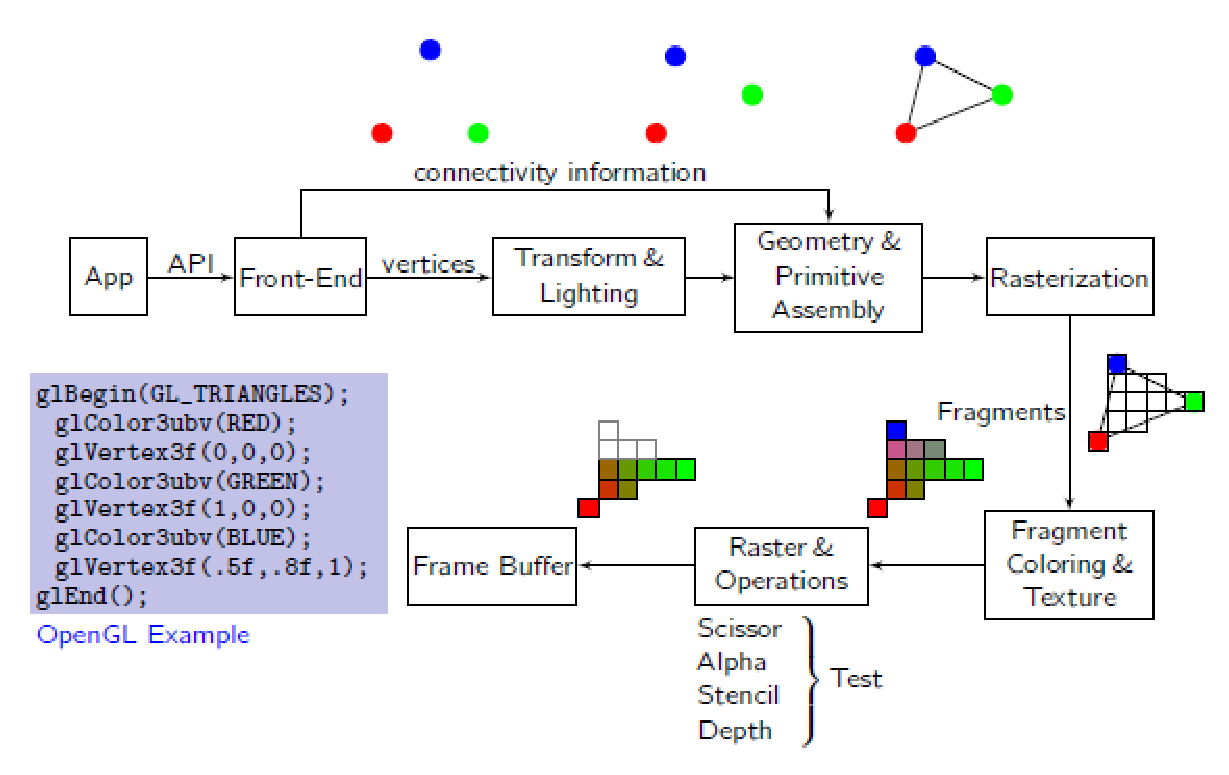
\includegraphics[height=8cm,
    angle=0]{./images/graphics_pipeline.eps}}
  \caption{Graphics pipeline}
  \label{fig:graph_pipeline}
\end{figure}



\subsection{Shaders: programmable GPU cores}
\label{sec:shader}

\begin{mdframed}

The rendering pipeline - Fig.\ref{fig:graph_pipeline} has many stages.
The rendering pipeline defines certain sections to be programmable. Each of
these sections, or stages, represents a particular type of programmable
processing. Each stage has a set of inputs and outputs, which are passed from
prior stages and on to subsequent stages (whether programmable or not).

\end{mdframed}

From recent GPU generations, the chips are programmable, i.e. each stage in the
rendering pipeline, Fig..\ref{fig:graph_pipeline}, is programmable.
Shaders are used to program what the GPU must do in each of the programmable
stages of the rendering pipeline.

A Shader is a user-defined program designed to run on some programmable stage of
a graphics processor. Shaders are written using {\it shading languages} like
Nvidia's Cg, OpenGL's GLSL (OGSL - Sect.\ref{sec:OGSL}), or Microsoft's HLSL.

So, a shader is a relatively small binary programs running on GPU.
Shaders controls either vertex, pixel or geometry processing. Also, a {\bf
shader process} is a small floating-point processor inside the GPU.

Shaders originated as small program that allowed tweaking the lighting
calculations for a surfade, aka "shading" objects. Eventually, shader support
was added to various parts of the fixed-function rendering pipelines inherent to
GL/D3D.


Shades fall into one of the following categories, depending upon its input
\begin{enumerate}
  \item Vertex Shaders: most established and common kind of 3D shader and are run once for each vertex given to the graphics processor.
  
  transform each vertex's 3D position in virtual space to the 2D coordinate at
  which it appears on the screen (as well as a depth value for the Z-buffer).
  
  CODE: apply the projection matrix (or, as optimization, hardcode the
  projection calculations required by your game).
  
  Vertex shaders can enable powerful control over the details of position,
  movement, lighting, and color in any scene involving 3D models.
  
  \item {\bf Pixel Shaders}: 
  
  \item {\bf Geometry Shader }
  
  \item {\bf Tessellation Shader}
\end{enumerate}
While shader stages do use the same language, each stage has a separate set of
inputs and outputs, as well as built-in variables.

With shader functions, the effects is limited by the programmer's imagination,
i.e. you have total control of how vertices and pixels are displayed. Given
that, using shader functions give more freedom to programmers. 


In 2002, with DirectX 8, it allows GPU programmers to program tailored
transformation and lighting calculations, as well as pixel coloring
functionality.

In 2002, DirectX 9 allows using much longer shader programs than before (pixel
and vertex shader 2.0) (Sect.\ref{sec:shader_model}). 

Shader source is compiled into bytecode offline, then transformed into a
GPU-specific binary by the graphics driver at runtime. \textcolor{blue}{Shader
functions may access (but not modify) large, globally shared data buffers}.
Prior to pipeline execution, these buffers are initialized to contain
shader-specific parameters and textures by the application.

At this time, graphics processors still has dedicated units for diverse types of
operations: vertex processing or pixel shading. Since DirectX 10, a unified
architecture was proposed. All hardware units are identical (with the name {\bf
shader processors} or stream processor), and can do the same thing.

With the birth of DirectX 11, a shader processor can be either pixel, vertex,
geometry and new is a compute shader (Chap.\ref{chap:DirectCompute}).


\url{https://www.khronos.org/opengl/wiki/Shader}



\subsection{HDR Texture Compression}
\label{sec:HDR_Texture_compression}

DirectX 11 supports new texture compression methods: BC6 and BC7. Block
compression 6 (BC6) compresses high dynamic range (HDR) data at a ratio of 6:1,
given hardware support for decompression. BC7 offers 3:1 compression ratios for
8-bit low dynamic range (LDR) data.  



\section{Evolution of GPU's capability}

In graphical applications, it's critical to achieve real-time
processing. Thus, to enhance the parallelism, many execution units are
added to the GPU chip, and the number of tasks done by the hardware in
GPU has been increased since then.  

Microsoft Direct3D\footnote{Direct3D is a part of DirectX} and OpenGL are
graphical standards with many 3D rendering APIs, Fig.~\ref{fig:direct3D}, that
use hardware acceleration. The GPUs that support these standards are known as 3D
GPUs.

\begin{figure}[hbt]
  \centerline{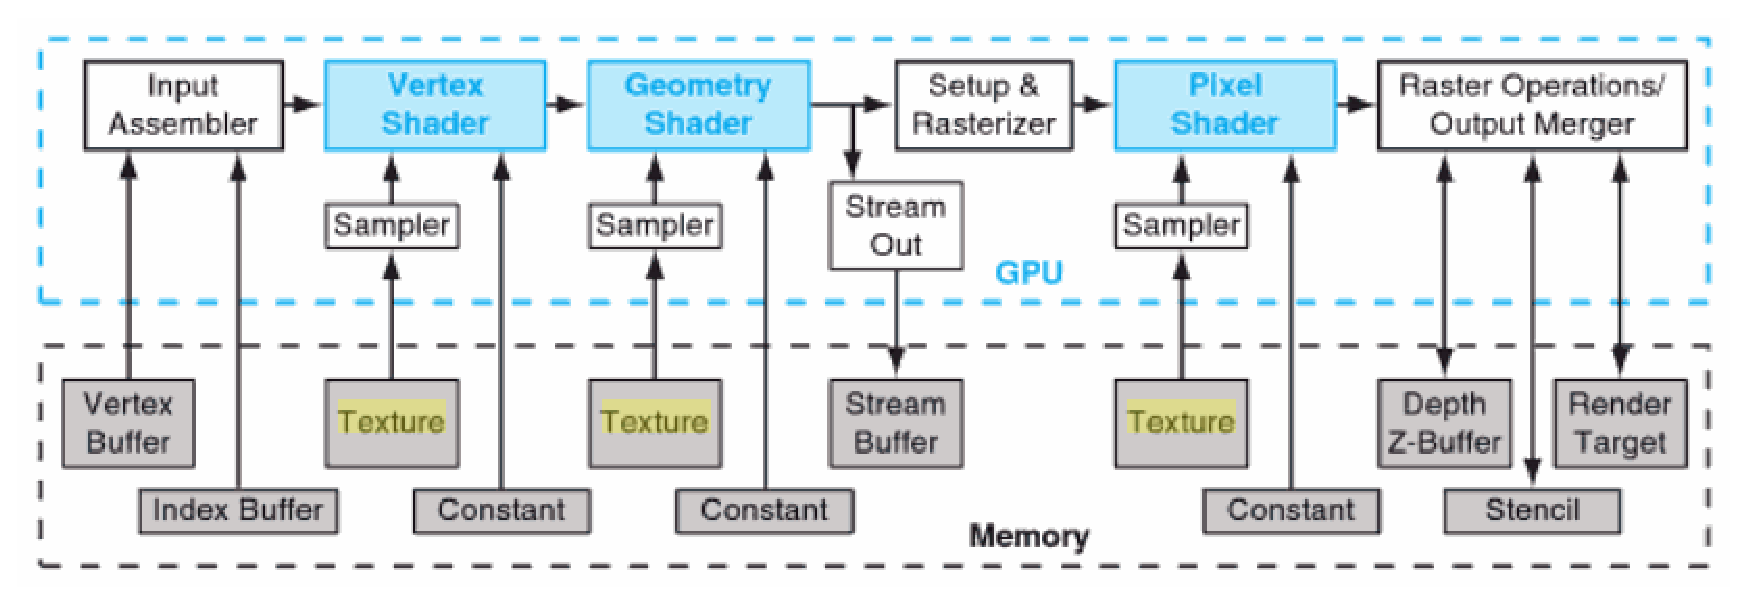
\includegraphics[height=5cm,
    angle=0]{./images/direct3D.eps}}
 \caption{Direct3D 10 graphics pipeline (OpenGL API has a similar structure)}
\label{fig:direct3D}
\end{figure}


Some of the important time-marks are given in
Fig.~\ref{fig:gen_of_GPU}.
\begin{itemize}
\item First generation of 3D GPU, chip 3dfx Voodoo: can do some tasks
  (e.g. rasterization), yet some need to be done on CPU, e.g. vertex
  transformations, texture mapping, z-buffering.
\begin{figure}[hbt]
  \centerline{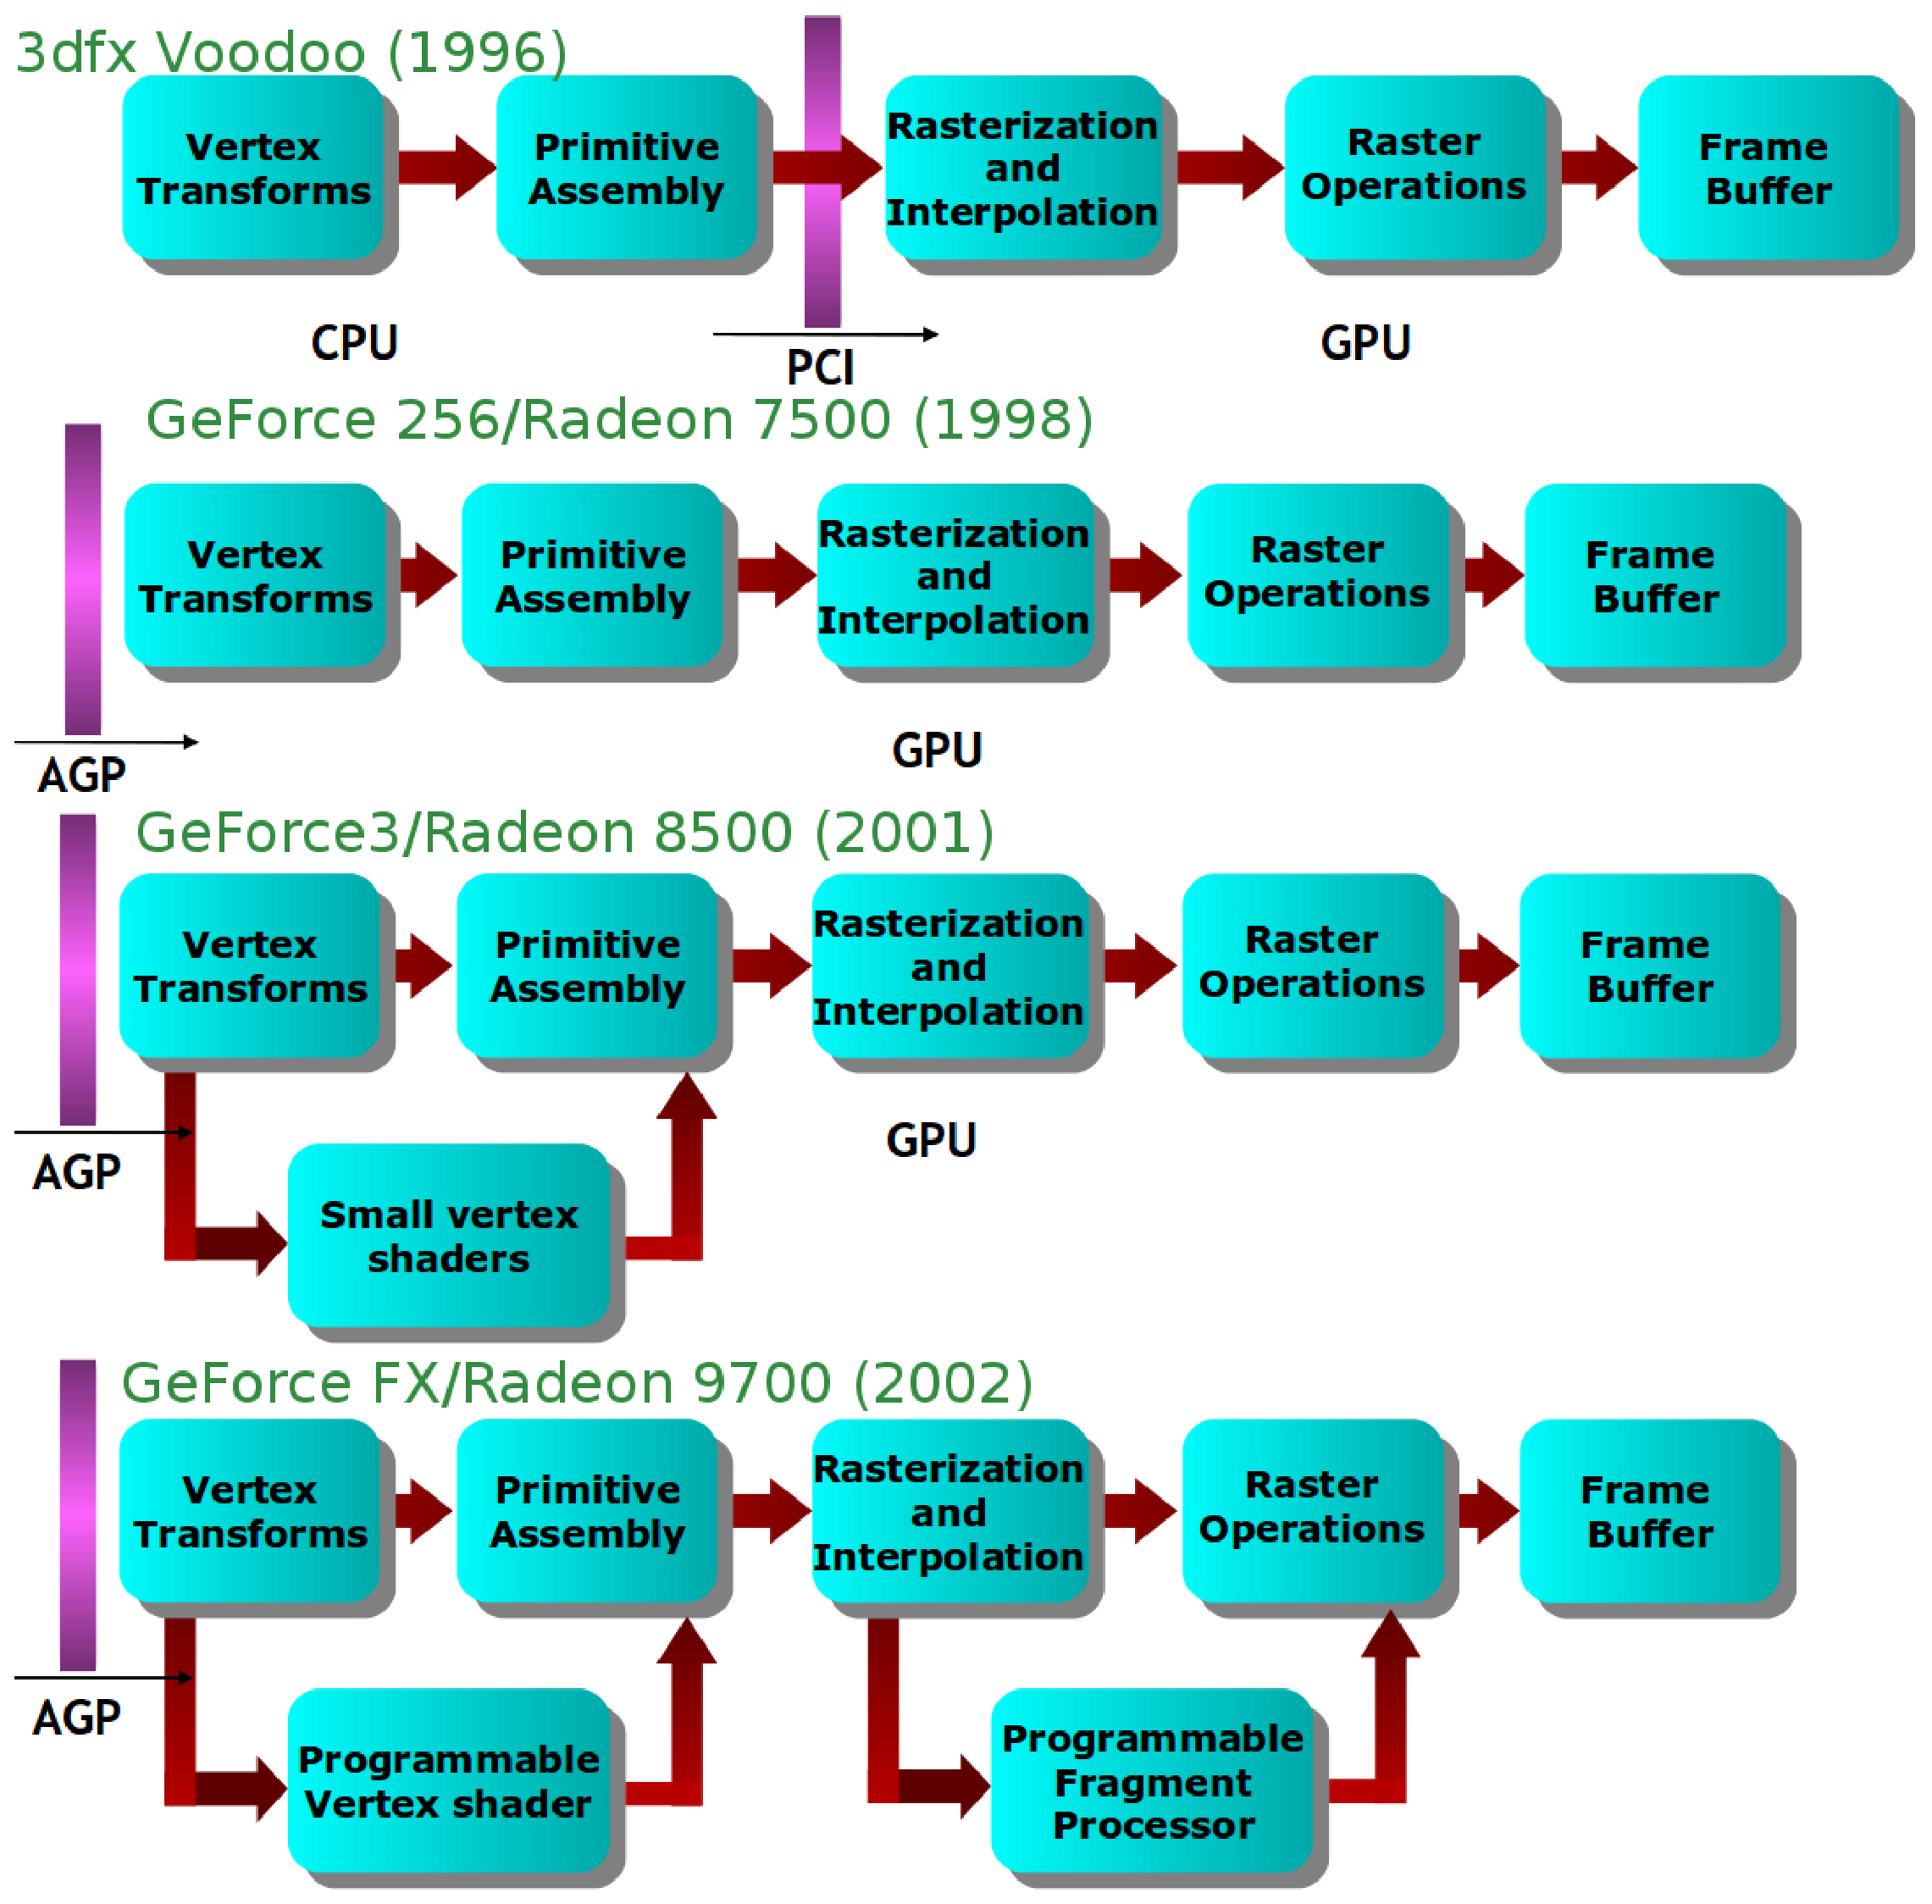
\includegraphics[height=7cm,
    angle=0]{./images/graphics_pipeline_2.eps}}
\caption{3D GPU (A) First Gen, (B) Second Gen, (C) Third Gen, (D) Fourth Gen}
\label{fig:gen_of_GPU}
\end{figure}

\item Second generation shift everything to GPU with faster bus (using
  AGP instead of PCI). It also have multi-texturing: giving bump maps,
  light maps, and others..

\item Third generation, for the first time, allows some limited amount
  of programmability on the vertex pipeline. It has multi-sampling
  (for antialiasing) and volume texturing. 

\item Fourth generation is the first generation of fully-programmable
  GPU. 
\item Fifth generation (Nvidia's G80) is the first one to fully
  support Direct3D 10 standard.
\end{itemize}


\begin{figure}[hbt]
  \centerline{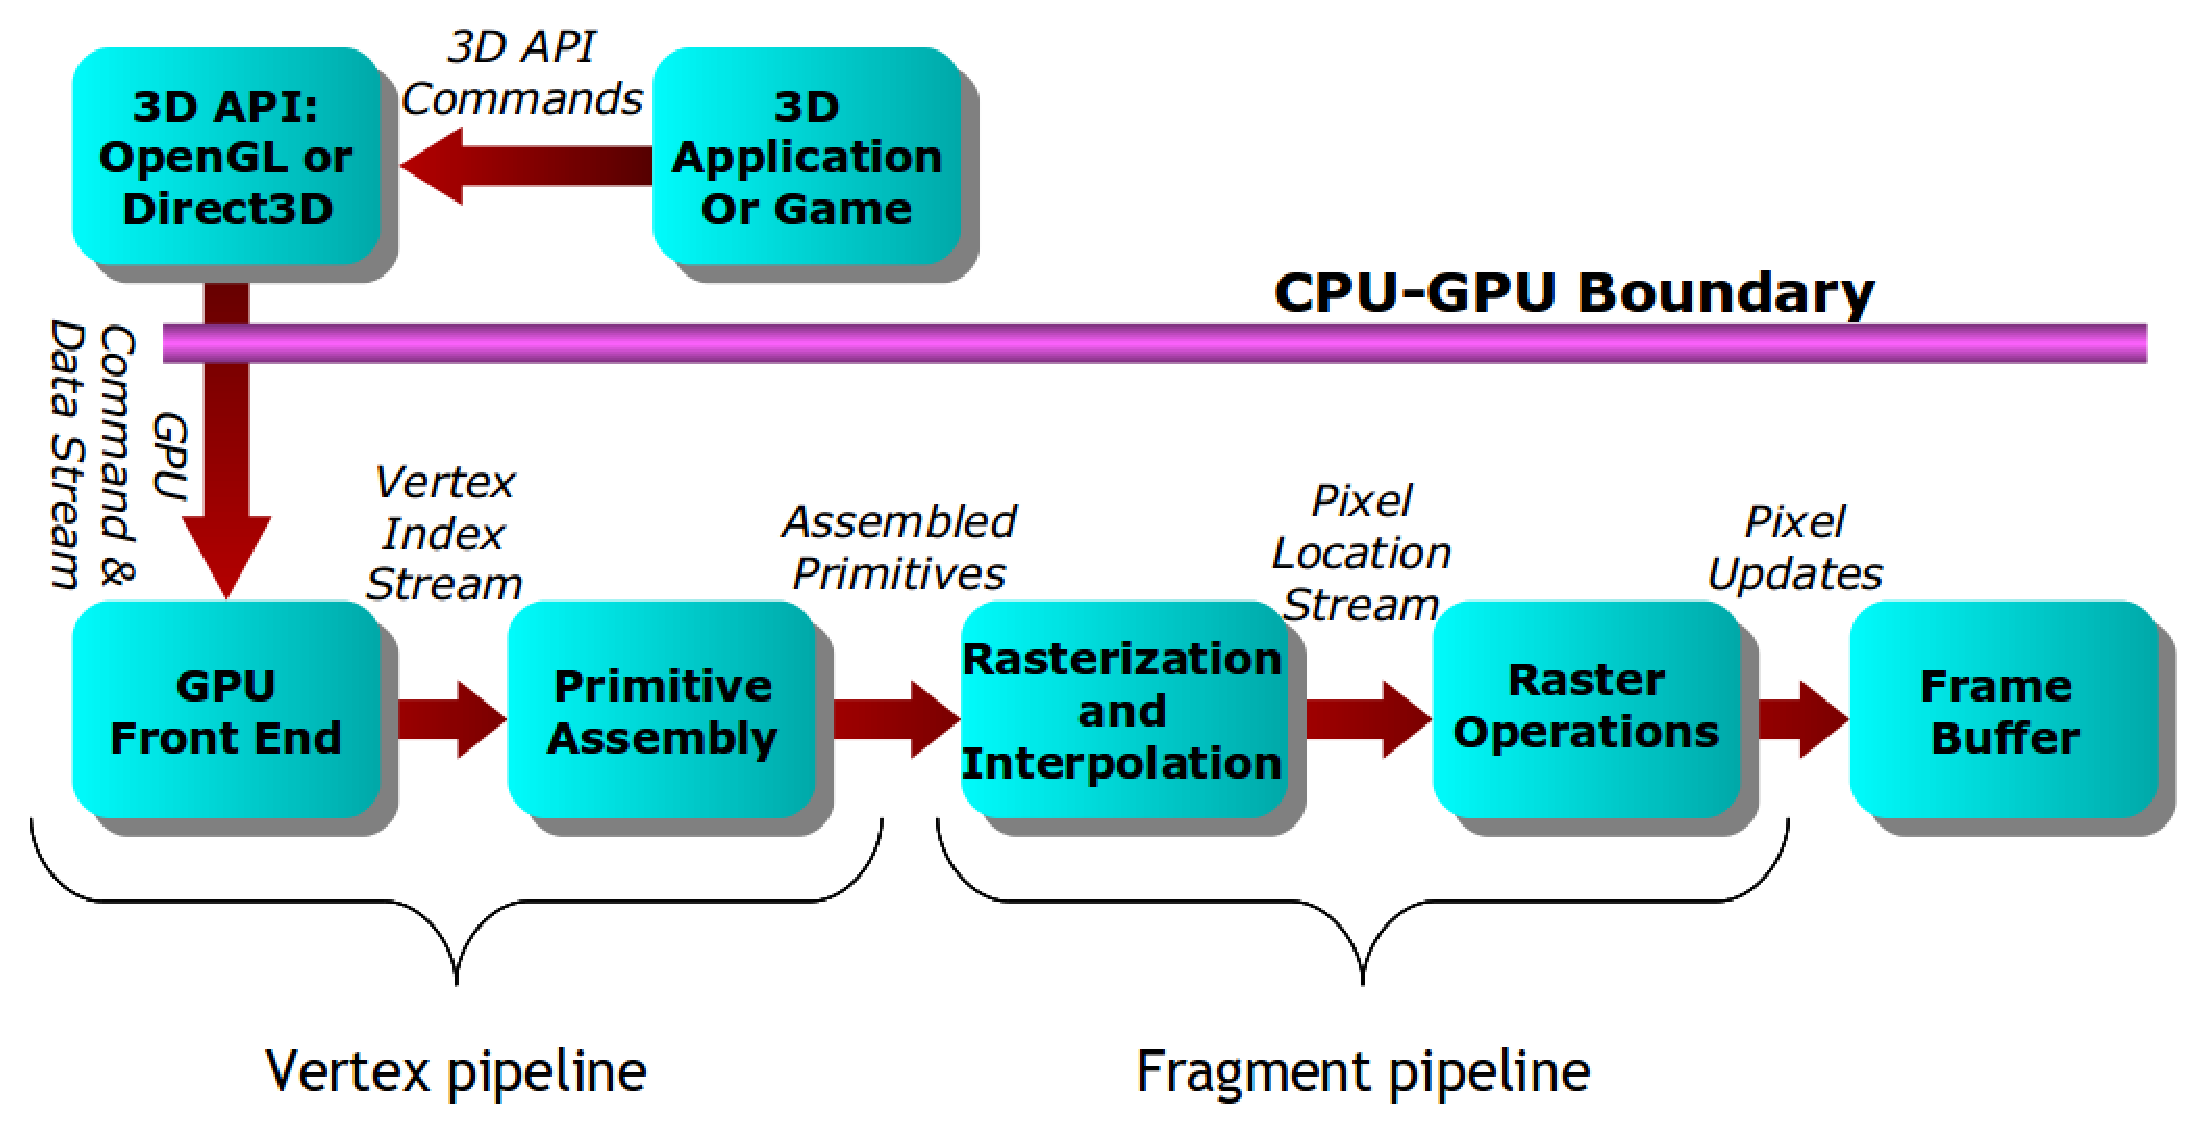
\includegraphics[height=5cm, angle=0]{./images/graphics_pipeline_3.eps}}
  \caption{Graphics pipeline}
  \label{fig:graph_pipeline_2}
\end{figure}

The hardware execution units that
are designed to process those tasks are called {\bf shaders} (or previously {\bf
  pipeline}). With two major data types ( pixel and vertex), shaders
are divided into two classes, 
Fig.~\ref{fig:graph_pipeline_2}: {\it 
  pixel-fragment shader} and {\it vertex
  shaders}~\footnote{\url{http://www.xbitlabs.com/articles/video/display/gf8800_3.html}}. 

\begin{enumerate}
\item Pixel-fragment shader: high-latency, low-precision texture
  filtering (to compute color for each pixel)

\item Vertex shader: low-latency, high-precision math operations
  (which thus become programmable first)
\end{enumerate}

The functions that run on theses shaders are also sometimes called
shaders as well, e.g. vertex shader, geometry shader, and fragment
shader, and can be written in
\begin{itemize}
\item Shader Assembly (ARB) - not widely used
\item Cg (C for graphics developed by Nvidia + Microsoft for
  programming vertex/pixel shaders)
\item GLSL (OpenGL Shading Language)
\item HLSL (Highe-Level Shading Language, i.e. DirectX, and only
  support DirectX APIs)
\item RenderMan (Pixar)
\end{itemize}
The output of the code written in these languages are the shader
programs to run on GPU.  So far, the processors run pixel shaders are
different from processors run vertex shader.
\textcolor{red}{Generally, GPUs process more pixels than vertex; thus
  the number of pixel shaders outnumbered vertex shaders, by a ration
  of about 3:1}.
Though this design has a number of advantage; it has some
drawbacks. The fact is that in some application, when we need more
vertex processing than pixel processing, we can not use free pixel
shaders for vertex processing.

\begin{figure}[hbt]
  \centerline{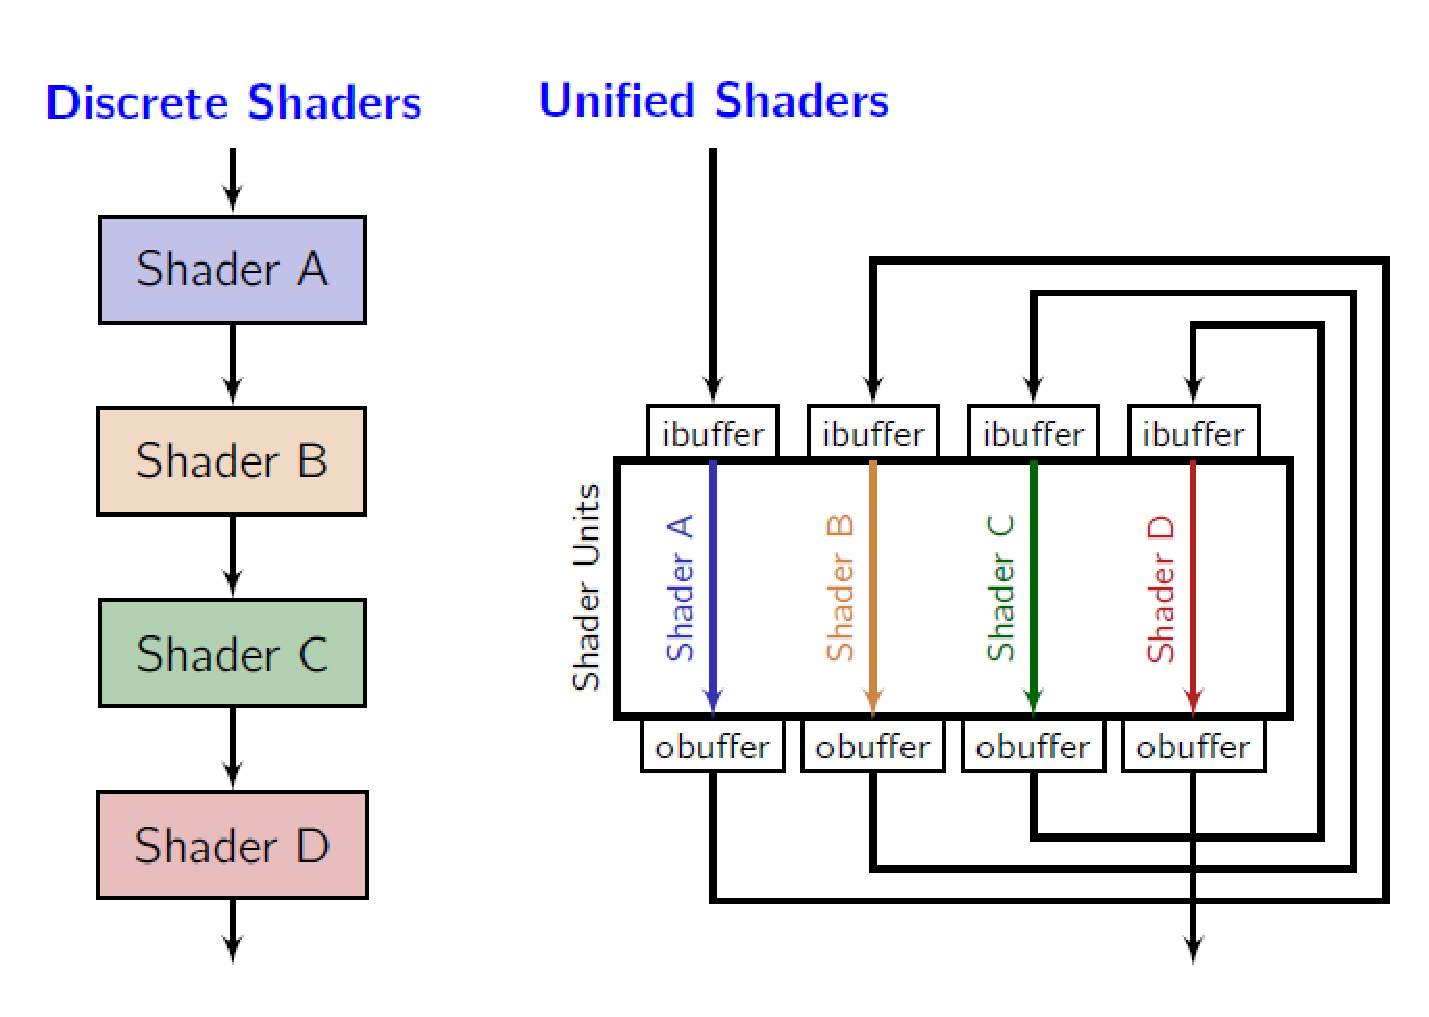
\includegraphics[height=5cm,
    angle=0]{./images/gpu_shader_1.eps}},
  \centerline{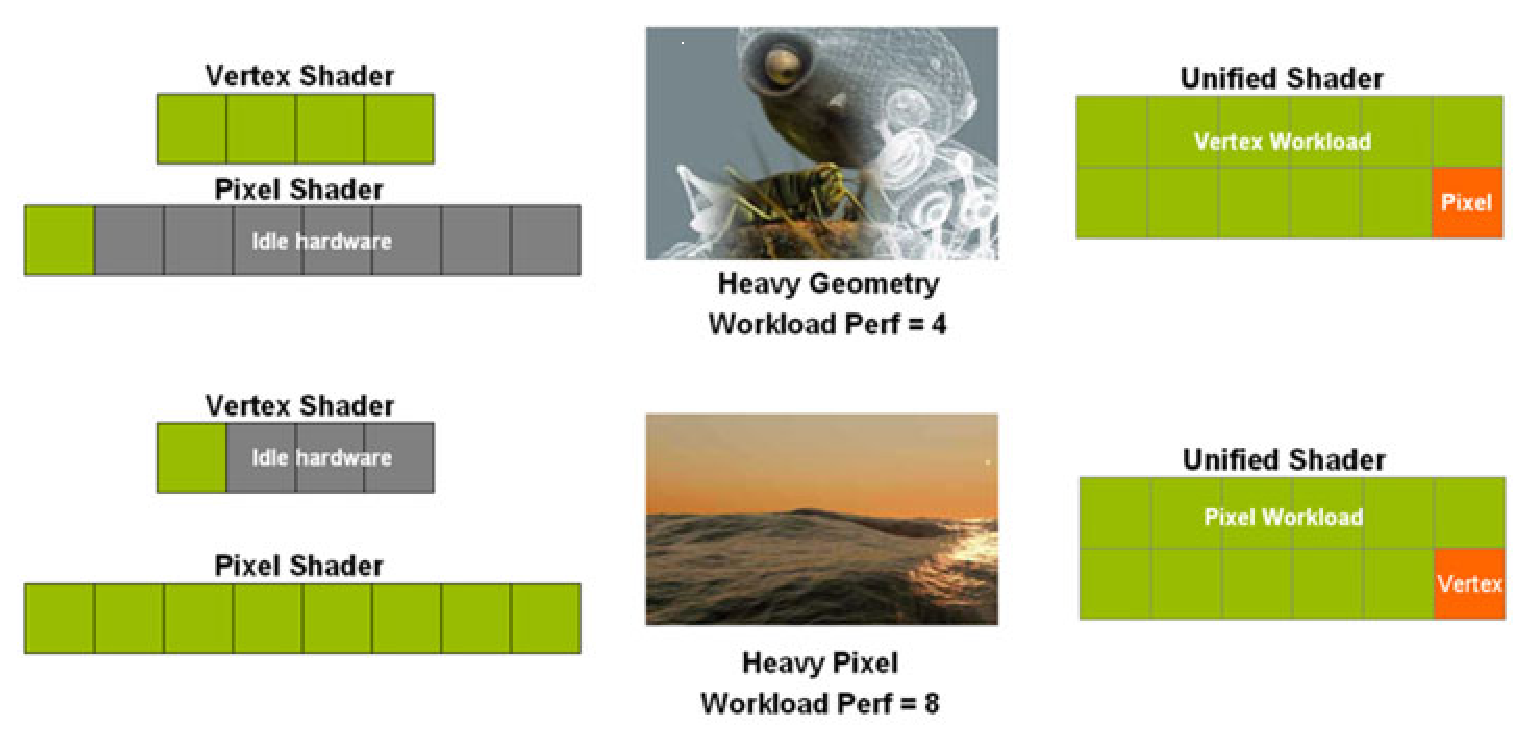
\includegraphics[height=5cm, angle=0]{./images/unified_shaders_2.eps}}
  \caption{Shaders and Unified Shader}
  \label{fig:shader_unified_shader}
\end{figure}

\textcolor{blue}{The concept of unified architecture allows the
  execution of vertex and pixel-fragment shaders on the same
  processor architecture}, rather than discriminated architecture,
  Fig.~\ref{fig:shader_unified_shader} and
  Fig.~\ref{fig:unified_shader}. This allows dynamic distributing the
  tasks to all processors, regardless of the type of the task. The new
  generation of GPU, unified architecture, build everything around the
  processors.  Using unified architecture, the idea of extending the
  application of GPU to GPGPU is given in Fig.~\ref{fig:GPU_GPGPU}

\begin{figure}[hbt]
  \centerline{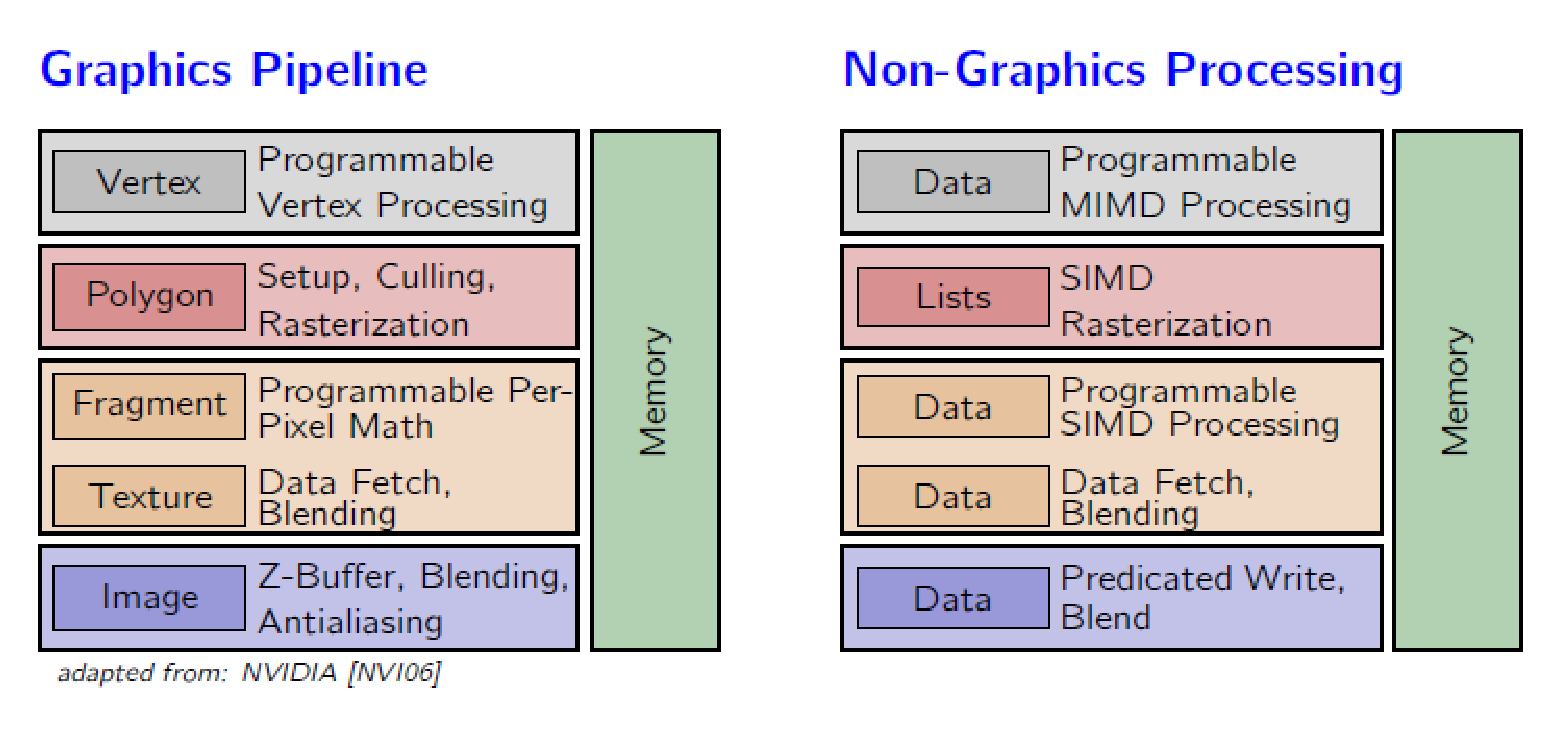
\includegraphics[height=5cm,
    angle=0]{./images/GPU2GPGPU.eps}}
  \caption{From GPU to GPGPU}
  \label{fig:GPU_GPGPU}
\end{figure}

\begin{framed}
  As the GPU instruction sets has evolved to the point that it is now
  possible to use the GPU for general purpose computations, Nvidia
  extend this unified architecture of GPU by building a new
  programming model that is easier for programmers. This is given the
  name CUDA (Compute Unified Architecture). In CUDA, shader is called
  scalar processor (SP).
\end{framed}


Based on the concept of unified architecture, in 2006, to help interacting with
GPU easier, a new set of APIs known as CUDA was developed (Sect.~\ref{sec:gpu-unif-arch}). It's an
extension of C language that allow user to write code running on GPU
easily for non-graphical applications. Nevertheless, there are
concepts derived from graphics application, so it's worthy to learn
some of them.

\section{ShaderModel specification}
\label{sec:shadermodel_specs}
\label{sec:shader_model}

As each gpu core process one instance of a shader (Sect.\ref{sec:shadermodel_specs})
GPU cores are called a shader. Before the invention of a unified architecture,
shaders are grouped into 3 categories: pixel shader, vertex and geometry shader.
So, if the binary program is supposed to run on a pixel shader, it's called a
pixel shader too. The shading language developed by Microsoft to use Microsoft
Direct3D API is called HLSL (high-level shading language). 

Shader Model 1 is the first shader model created in DirectX, with vertex and
pixel shaders, to allow programmers to code a shader using HLSL. A binary
program can be classified into either a pixel shader, vertex shader or geometry
shader.


Intrinsic function is Shader Model 1.1:
\url{http://msdn.microsoft.com/en-us/library/windows/desktop/ff471376(v=vs.85).aspx}

Shader Model 2.0 add more functions to Shader Model 1.0. 

Shader Model 3.0 add more functions to Shader Model 2.0.

Shader Model 4.0 add more functions to Shader Model 3.0, and remove support for
features in Shader Model 1.0. Here, all shaders are treated the same, using
common-shader core. Also, a new pipeline stage is added (geometry-shader stage),
to create or modify an existing geometry. 

Shader Model 5.0 add more functions to Shader Model 4.0, with double-precision
support (to support better polymorphism, objects, and interfaces). A new shader
({\bf compute shader}) is added to provide high-speed general purpose computing.
A compute shader is a programmable shader that expand Microsoft Direct3D 11
beyond graphics programming. This is known as {\bf DirectCompute} technology
(Chap.\ref{chap:DirectCompute}).


References:
\begin{itemize}
\item Computer organization and design: the hardware/software interface
  By David A. Patterson, John L. Hennessy - Appendix A. 
\item \url{http://www.behardware.com/articles/644-3/Nvidia-geforce-8800-gtx-8800-gts.html}
\item
\url{http://msdn.microsoft.com/en-us/library/windows/desktop/ff476331(v=vs.85).aspx}
\end{itemize}



\section{HLSL}
\label{sec:HLSL}

HLSL is developed and maintained by Microsoft, and the APIs library is Microsoft
Direct3D. Using HLSL, you can write one of the 4 different forms of code:
\begin{enumerate}
  \item vertex shaders
  \item geometry shaders
  \item pixel (fragment) shaders
  \item compute shaders
\end{enumerate}

\section{ OpenGL Shading Language (GLSL)}
\label{sec:OGSL}
\label{sec:GLSL}

To give the programmers the freedom of coding their program running on GPU like
a binary running on CPU, shading languages were developed. 

GLSL is developed and maintained by OpenGL ARB community, and the APIs library
is OpenGL. 

